\documentclass[11pt]{article}

\usepackage[a4paper, total={6in, 8in}]{geometry} % page layout
\usepackage{booktabs} % table
\usepackage{longtable} % longtable
\usepackage{kotex} % Korean
\usepackage[round,colon,authoryear]{natbib} % Reference
\usepackage{graphicx}
\usepackage{url}
\usepackage{float}


\begin{document}           

    \title{Project Proposal: Vertiport Placement in Gyeongsangbuk-do and Daegu through K-Means Algorithm for Middle Mile Logistics Optimization}          
    \author{
        Chungho Park\textsuperscript{a},
        Juchan Lee\textsuperscript{a},
        Yoobin Park\textsuperscript{a},
        Shinkook Cha\textsuperscript{a},
        Yujin Kim\textsuperscript{a},
        Junghyun Kim\textsuperscript{a}\\
        {\small \textsuperscript{a}School of Applied Artificial Intelligence, Handong Global University}\\
        {\small 558 Handong-ro, Pohang-si, Gyeongbuk, South Korea}\\
    }

    \date{Fall Semester, 2023}      

 
    \maketitle                 
 
    \begin{abstract}
        With rapid urbanization and an increase in city population, conventional modes of transportation are facing critical limitations: high CO2 emission, congestion costs, air pollution, etc. In order to tackle this problem, a new mode of air transportation, namely Urban Air Mobility (UAM), has been introduced. However, one of the greatest hurdles behind the implementation of UAM is the selection of appropriate vertiport locations (i.e., vertiport placement). Thus to overcome the vertiport placement problem, we propose a pipeline of collection, preprocessing, and integration of the datasets and clustering by the K-Means algorithms to select vertiport placement locations for better efficiency of the fresh food middle-mile delivery in Gyeongsangbuk-do and Daegu. 
    \end{abstract}

    \tableofcontents
    \newpage
    
    \section{Introduction} 
    \subsection{Project background}
    With the rise in population and rapid urbanization, contemporary cities grapple with challenges such as traffic congestion and increased CO2 emissions \citep{LeeHong2021}. In response to these issues, a revolutionary mode of transportation has emerged – Advanced Air Mobility (UAM), more specifically UAM, a subset of UAM, characterized by safe, efficient, and sustainable air transportation, which shows contrast to conventional helicopters\citep{LeeHong2021, YunLeeHwang2019}; and due to these traits, the UAM represents a paradigm shift, enabling swift movement within city centers and between nearby cities where traditional air transport services were unavailable \citep{JungYuYun2021}.
    
    While UAM offers a promising alternative to ground transportation, it confronts challenges. Investment in UAM faces barriers such as policy considerations, noise regulations, aviation methods, and potential issues with aircraft production and electric batteries. For instance, overcoming airspace barriers involves addressing route planning and integrating UAM systems with existing air transportation infrastructure is a critical issue \citep{KimKim2023}. However, amongst many other challenges that the implementation of UAM faces, determining the optimal locations for UAM vertiports—designated take-off and landing sites—is a particularly significant consideration that demands time and financial investment.

        \begin{longtable}[c]{@{}lllll@{}}
    \caption{Previous Studies}
    \label{tab:my-table}\\
    \toprule
    Author(year) & Research Purpose & Considered Variables \\* \midrule
    \endfirsthead
    %
    \endhead
    %
    \bottomrule
    \endfoot
    %
    \endlastfoot
    %
    Moon et al (2021) & \parbox[t]{5cm}{Identifying the Potential Vertiport Location for Addressing Traffic in the Busan Area\citep{MoonShiKang2021}} & \parbox[t]{5cm}{\raggedright Transportation connectivity, Workplace density, Official land price, Number of commuters, Estimated income quintile, Average transportation cost, Parking lot accessibility, Residential density, Noise\\} \\
    Sung et al (2023) & \parbox[t]{5cm}{Optimal Location Selection and Efficiency Analysis of Driving Route Travel Time for Practical Use of Vertiport\citep{SungKimChoiCho2023}} & \parbox[t]{5cm}{\raggedright Airspace restriction area, Natural environment conservation area, river, Public transportation demand, Living population density, Average annual income, Individual official land price, Transportation connection, Residential density\\} \\
    Jeong and Hwang (2021) & \parbox[t]{5cm}{Analysis of demand for eVTOL to reduce commuting time in the Seoul metropolitan area and selection of vertiport location\citep{JeongSoHwang2021}} & \parbox[t]{5cm}{\raggedright Commuting population, Green belt, Airspace restriction area, Residential area\\} \\
    Kim et al (2023) & \parbox[t]{5cm}{Suggesting the direction of vertiport construction to increase usage through analysis in terms of usage environment\citep{kim-2023}\\} & \parbox[t]{5cm}{\raggedright Accessibility, Affordability, Living environment\\}  \\
    Jung et al (2021) & \parbox[t]{5cm}{Deriving Vertiport Location Selection Factors and Analysis of Location Assessment Factors \citep{JungYuYun2021}\\} & \parbox[t]{5cm}{\raggedright Land costs, Transportation connectivity, Obstacles, Ease of supply and construction of power sources, Noise environment, Law\\} \\
    Son et al (2023) & \parbox[t]{5cm}{Selecting the location of the vertiport in the Seoul metropolitan area, building a network, estimating usage, and calculating the scale of the vertiport \citep{Son-2023}\\} & \parbox[t]{5cm}{\raggedright Traffic volume} \\
    
    Min et al (2020) & \parbox[t]{5cm}{Select a vertiport construction area in Seoul by analyzing the composition of physical infrastructure and considerations by type \citep{Min-2020}\\} & \parbox[t]{5cm}{\raggedright Airspace restriction area in Seoul, Floating population, Connection of ground transportation} \\* \bottomrule
\end{longtable}
 

    In addition, despite the ongoing discussions to resolve these challenges, the majority of studies thus far have focused on UAM as simply a mode of human transportation. However, according to the K-UAM Roadmap, logistics transportation is anticipated to be commercialized decades faster than human transportation due to differences in safety requirements, supporting the rationale behind utilizing UAM as a mode of logistics before human transportation. Especially, in light of the recent relocation of Daegu Airport to the Gunwi area (new TK airport), the establishment of a new airport logistic network is being underscored and accentuated, emphasizing the even greater critical role of optimal vertiport placement in logistics to ensure its success.
    
    Due to these reasons - vertiport placement problem and UAM network establishment in logistics - our project narrowed down the focus to the realm of logistics transfer, with a particular emphasis on fresh food delivery. This choice is informed by several pressing issues, including the substantial economic losses incurred by Gyeongsangbuk-do in 2018 due to traffic congestion costs \citep{congestion}, frequent delivery delays, and inadequate temperature control, which in turn leads to the increased risk of lowered food quality \citep{quick_logistic, latency_logistic} and finally, challenges that persist in delivering to mountainous regions \citep{ChoiOh2011}.
    
    In light of these challenges and the growing need for efficient and sustainable logistics solutions, the project seeks to address the optimal placement of vertiports for fresh food delivery. 
    
    \subsection{Research question}

    \begin{itemize}
        \item \emph{RQ 1: "What constraints should be considered to operate UAM?"
        }
         
        \item \emph{RQ 2:  "What constraints should be considered to build a vertiport"}

        \item \emph{RQ 3: "How can we infer logistics demand when we do not have a dataset that directly reflects logistics demand?"
        }

        \item \emph{RQ 4: How can we validate our findings? (i.e., How can we validate that the selected veriport locations are optimal?)
        }
        

    \end{itemize}


    \subsection{Project goal}
    The goal of our project is to select optimal vertiport locations in Gyeongsangbuk-do for logistics purposes. Variables that affect optimality and feasibility such as restricted air spaces, logistics demand, logistics warehouse volume, and ground slope will be taken into account. By having demand visualized as dotted points on a 2D plane, we will utilize the K-Means clustering algorithm to cluster the points into K different clusters. We expect to have centroid points of the clusters as near-optimal vertiport locations and the exact locations will be later fine-tuned with real-life restrictions and limitations taken into consideration. By doing so, we expect the selected vertiport locations to facilitate air-traveled logistics and reduce the middle-mile delivery time of fresh foods. 
   
    \section{Project Design}
    \subsection{Project plan}                       
    \begin{longtable}[c]{@{}lllll@{}}
    \caption{Project Plan}
    \label{tab:my-table}\\
    \toprule
    Week & Plan & Contents \\* \midrule
    \endfirsthead
    %
    \endhead
    %
    \bottomrule
    \endfoot
    %
    \endlastfoot
    %
    Week 9 & Midterm project presentation feedback & \parbox[t]{6cm}{\raggedright Received \& reflected feedback for the midterm presentation from technical advisor Youngjae Lee and professor Junghyun Kim.\\ } \\
    Week 10 & Hypothesising down topic & \parbox[t]{6cm}{\raggedright Revised the topic and conducted background research.\\ 
    Listed up features to consider for the research regarding Advanced Air Mobility and middle-mile delivery system.\\}\\
    Week 11 & \parbox[t]{6cm}{Data collection, preprocessing, and Visualization} & \parbox[t]{5cm}{\raggedright Collected and visualized airspace by matplotlib(Python). \\ 
    Collected and visualized restricted slope by QGIS.\\ } \\
    Week 12 & \parbox[t]{6cm}{Data collection, preprocessing, and Visualization} & \parbox[t]{6cm}{\raggedright Collected and visualized Gyeonsangbuk-do and Daegu boundary data by matplotlib(Python). \\ 
    Integrated slope data (QGIS) to matplotlib(Python) map.\\ 
    Collected Hwaseong lastmile delivery volume.\\ }  \\
    Week 13 & \parbox[t]{6cm}{\raggedright Data collection, preprocessing, and Visualization \\ Hypothesis Formulation} & \parbox[t]{6cm}{\raggedright Collected and visualized warehouse locations in Gyeonsangbuk-do and Daegu.\\
    Formulated hypothesis 1 to estimate the mathematical relationship between the warehouse and its width.\\ 
    Formulated hypothesis 2 to estimate efficiency of middle-mile delivery by AAM.\\ } \\
    Week 14 & \parbox[t]{6cm}{\raggedright Implementation of K-means algorithm \\ Preparation for final presentation\\} & \parbox[t]{6cm}{Implemented K-means algorithm and investigated selected candidate locations\\} \\
    Week 15 & \parbox[t]{6cm}{\raggedright Validation of hypothesis 1 \& 2 \\ Final Presentation}& \parbox[t]{6cm}{\raggedright Validated hypothesis 1 by clustering Hwaseong lastmile delivery data and estimated the relationship between delivery volume and warehouse width using linear regression. \\
    Validated hypothesis 2 by using KaKao navigation to estimate the efficiency of middle-mile delivery by AAM.\\} \\* \bottomrule
\end{longtable}
   
    \subsection{Project participants}                       

    \begin{longtable}[c]{@{}lllll@{}}
    \caption{Project participants}
    \label{tab:my-table}\\
    \toprule
    Name & StudentID & Major & email address & Language \\* \midrule
    \endfirsthead
    %
    \endhead
    %
    \bottomrule
    \endfoot
    %
    \endlastfoot
    %
    Sangsan Lee & 222000001 & Mechanical Engineering & ssl@handong.edu & Python \\
    Jaeyoung Chun & 222000002 & Bio-Informatics & jyc@handong.edu & Python, SQL \\
    Junghyun Kim & 222000003 & Aerospace & jhk@handong.edu & Python, C \\
    Keungoui Kim & 222000004 & Economics & kko@handong.edu & Python, R \\* \bottomrule
\end{longtable}
   

    \section{Data}
    \subsection{Data resource}
    
    In this research, data related to considerations for selecting vertiport locations for fresh food delivery using UAM in Daegu and Gyeongsangbuk-do were utilized.\
    
    First, to represent the target area of this research, Daegu and Gyeongsangbuk-do, the administrative division data of South Korea were collected. This data was obtained from the website GIS DEVELOPER operated by Geo Service Co., Ltd. The data is provided in the shapefile format and delineates administrative divisions from city and province levels to detailed town, village, and neighborhood units.\
    
    Second, to incorporate constraints about vertiport location selection, South Korea's airspace data and ground slope data were collected. Specifically, the no-fly zones, restricted areas, and danger areas were collected from the national spatial information platform "V-World" using the platform's open API to collect data in JSON format. These datasets were utilized to represent areas in Daegu and Gyeongsangbuk-do where UAM flights and vertiport placements are restricted. Another variable that was taken into consideration was the ground slope. According to EASA (European Union Aviation Safety Agency) \citep{unknown-author-2022} guidelines on vertiport designs, the slope of the OLS (Obstacle Limitation Surfaces) should be less than 50\%. To take ground slope into account during the vertiport selection procedure, we utilized Korea's ground slope data provided by the 'Korea Institute of Geoscience and Mineral Resources', and filtered out regions with ground slope levels higher than 50\% using the QGIS program. Gyeongsangbuk-do regions with airspace information and ground slope levels lower than 50\% have been visualized by the Matplotlib library (Fig. 1).
    
    \begin{figure}[H]
        \centering
        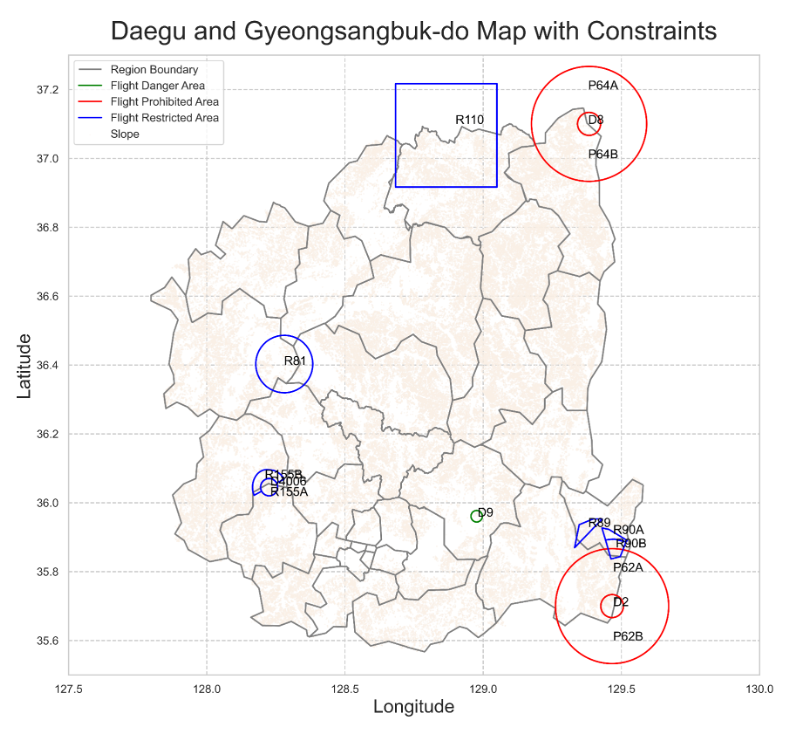
\includegraphics[width = 10cm]{./figure/airspace_and_groundslope.png}
        \caption{Airspace and Ground Slope in Daegu and Gyengsangbuk-do}
        \label{fig:enter-label}
    \end{figure}
    
    Third, to reflect the use of UAM as the fresh food delivery vehicle, warehouse location and volume data for the Daegu, Gyeongsangbuk-do, and Gyeonggi-do were collected. These data, which provide warehouse information at the city and province levels, were obtained from the National Logistics Information Center. The data for the Daegu and Gyeongsangbuk-do were collected for the selection of actual vertiport locations, while data of Gyeonggi-do were collected to estimate the relationship between warehouse area and logistics movement volume.
    
    Lastly, to estimate the relationship between warehouse volume and logistics movement volume in the Hwaseong region, last-mile data were acquired from CJ Logistics.


    \subsection{Data pre-processing}
    Since vertiport placement was conducted only for Daegu and Gyeongsangbuk-do, we removed administrative division data that were not a part of Daegu and Gyeongsangbuk-do. We applied the same process to the airspace and ground slope data.
    
    Regarding the area of the warehouse in Hwaseong, we considered only the data on the warehouse owned by CJ Logistics for comparison with the last-mile data of CJ Logistics.

    In addition, the warehouse area and the last mile data of the Hwaseong showed that the location information was stored as a lot number or road name address. It was necessary to convert location information into latitude and longitude coordinates for visualization purposes. Thus, we used the Geocoding API service of the Naver cloud platform. In this process, we removed items that were not converted to latitude and longitude coordinates due to incorrect address entries.

    \subsection{Data management}
    All data except ground slope data and CJ Logistics data are available in the GitHub URL below:\
    
    \url{https://github.com/HowveYoobin/Big_Data_Design/Team_project/data}\

    The ground slope data could not be uploaded to Github due to its large file size.

    \section{Method}                       
    \subsection{Methodologies}

    In this study, we employed the K-Means algorithm to select vertiport locations in Daegu and Gyeongsangbuk-do. The K-Means algorithm is a partitioning-based clustering algorithm, a type of unsupervised learning used to group given data into K clusters. Each cluster is characterized by a representative point called a centroid, and each data point is assigned to the nearest centroid. This algorithm forms clusters by minimizing the distance between the centroids and individual data points.\

    The procedure of the K-Means algorithm is as follows:\\

    Step 1. Specify the number of clusters and set initial centroids.
    
    Step 2. Assign each data point to the nearest centroid.
    
    Step 3. Update centroids to the mean points of data points in each cluster.
    
    Step 4. Repeat Steps 2 and 3 until centroids converge.
    
    Step 5. Terminate the algorithm when centroids converge.\\

    There are two reasons for choosing the K-Means algorithm among the various clustering algorithms available. Unlike density-based algorithms (e.g., DBSCAN), partitioning-based algorithms, such as K-Means, allow the user to specify the number of clusters. This means that the algorithm does not determine the number of clusters on its own; instead, users can make informed decisions based on real-world considerations, adjusting the number of clusters to align with the actual scenario. This flexibility in determining the cluster number allows the methodology to be adapted to real-world scenarios, allowing adjustments according to the practicalities of the introduction of UAM.
    
    Second, unlike other partitioning-based algorithms that assume specific data distributions (e.g., Gaussian Mixture Model with Expectation-Maximization), the K-Means algorithm relies on its distance-based approach to forming clusters. In the context of optimizing the middle mile, the focus is on finding the optimal locations for vertiports in proximity to warehouses rather than assuming a specific distribution of warehouse locations. This consideration led to the choice of the K-Means algorithm.


    \subsection{Analytic process}
    
    First, the administrative boundary of Daegu \& Gyeongsangbuk-do excluding Ulleung-do, and the new TK airport (i.e., Gunwi airport) location were visualized by the Matplotlib for spatial analysis. To visualize the constraints on vertiport placement, airspace including flight-restricted, -prohibited, and -danger areas was presented on the map by matplotlib. According to the EASA vertical take-off and landing procedure, take-off \& landing available areas (slope ${<}$ 0.5)  were marked on the map by Matplotlib. Then, refrigerated warehouse locations were marked on the map. We increased the number of points plotted on warehouse locations proportional to their respective width according to their positive correlation between width and transportation volume (Fig. 2).

    \begin{figure}[H]
        \centering
        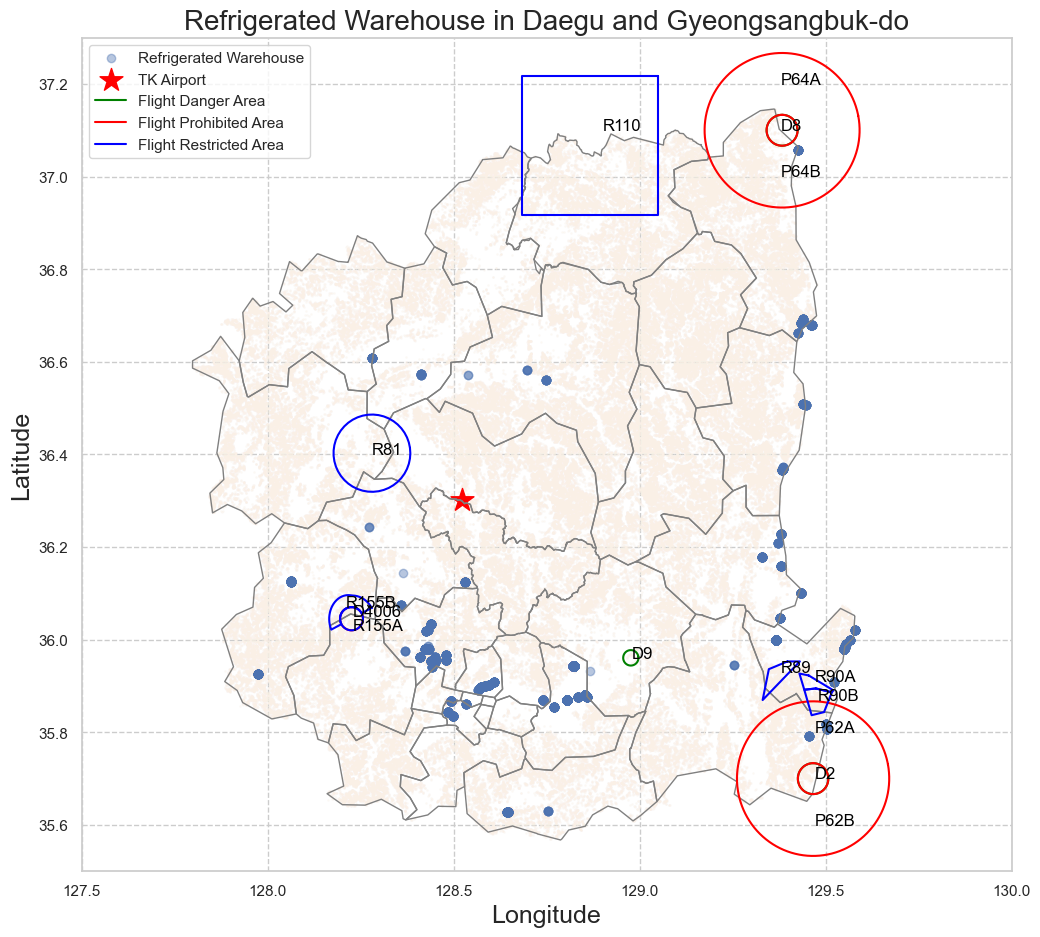
\includegraphics[width = 10cm]{./figure/basic.png}
        \caption{Airspace, slope, new TK airport, and refrigerated warehouse in Daegu and Gyeongsangbuk-do}
        \label{fig:enter-label}
    \end{figure}
    
    Before implementing the K-means algorithm, the number of clusters was predetermined by eye inspection, Silhouette method, and elbow method. Through the eye inspection, the visible number of clusters K was 3, and both of silhouette method and elbow method indicated 2 as the optimal K with a silhouette score of 0.677 (Fig. 3).
    
    \begin{figure}[H]
      \centering
      \begin{minipage}{0.32\textwidth}
        \centering
        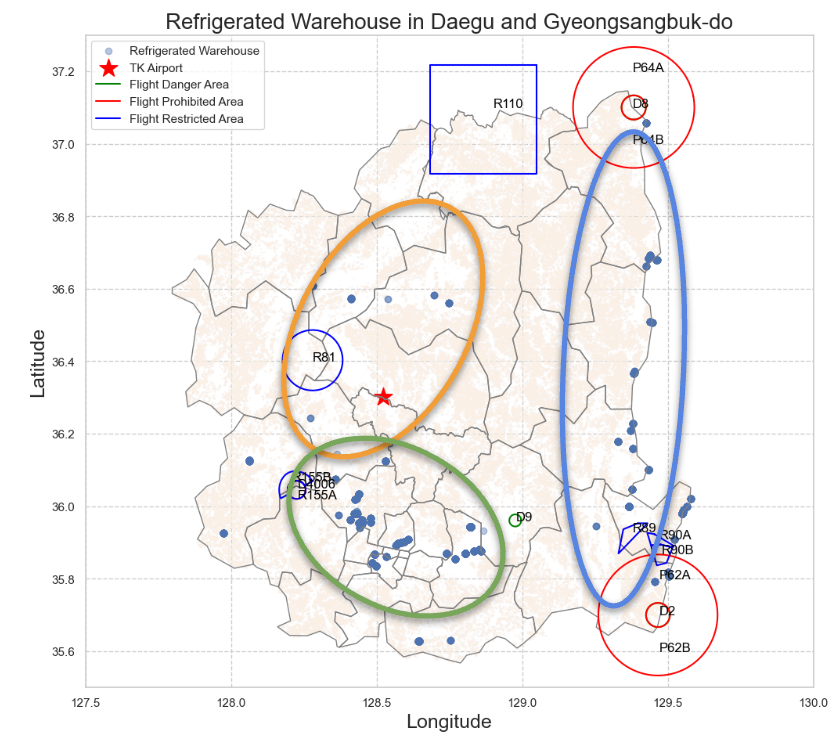
\includegraphics[width=\linewidth]{figure/eye_inspection.png}
      \end{minipage}%
      \begin{minipage}{0.32\textwidth}
        \centering
        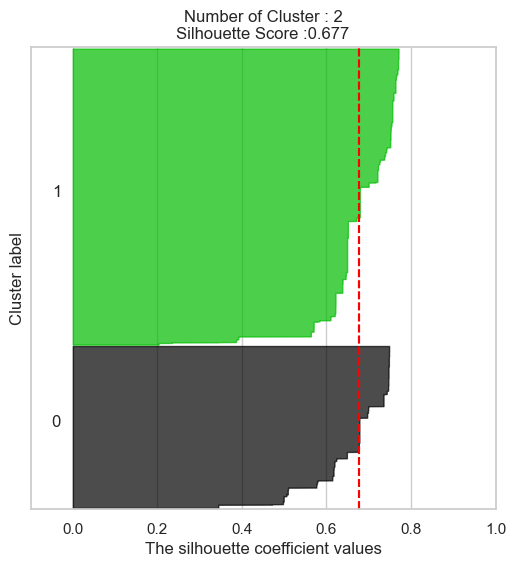
\includegraphics[width=\linewidth]{figure/silhouette_2.png}
      \end{minipage}%
      \begin{minipage}{0.32\textwidth}
        \centering
        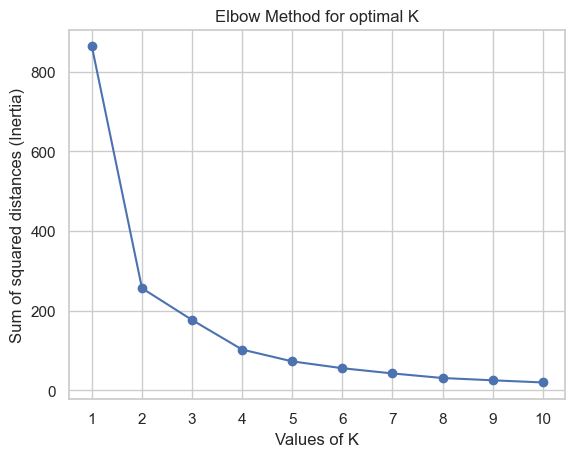
\includegraphics[width=\linewidth]{./figure/elbow.png}
      \end{minipage}
      \caption{Methods used to determine the number of clusters }
      \label{fig:overall}
    \end{figure}
    
    The K-Means algorithm was implemented with K = 2 and K = 3, respectively. The resulting centroids were selected as vertiport candidates, and the points were adjusted to their closest warehouse to guarantee their ground traffic connectivity. To guarantee that the vertiport candidates avoid any flight constraints, the vertiport candidate points were adjusted to the next closest warehouse if the adjusted centroids overlapped with flight-restricted areas. If the adjusted centroid does not overlap with any flight-restricted areas, its slope was checked to guarantee the vertiport candidate avoids take-off. If the location’s slope was lower than 0.5, the vertiport candidate location was adjusted to its closest location with a safe slope (slope ${>}$ 0.5). Then the selected vertiport locations were investigated closely by Google Maps satellite image (Fig 4, 5).\\

    \begin{figure}[H]
      \centering
      \begin{minipage}{0.5\textwidth}
        \centering
        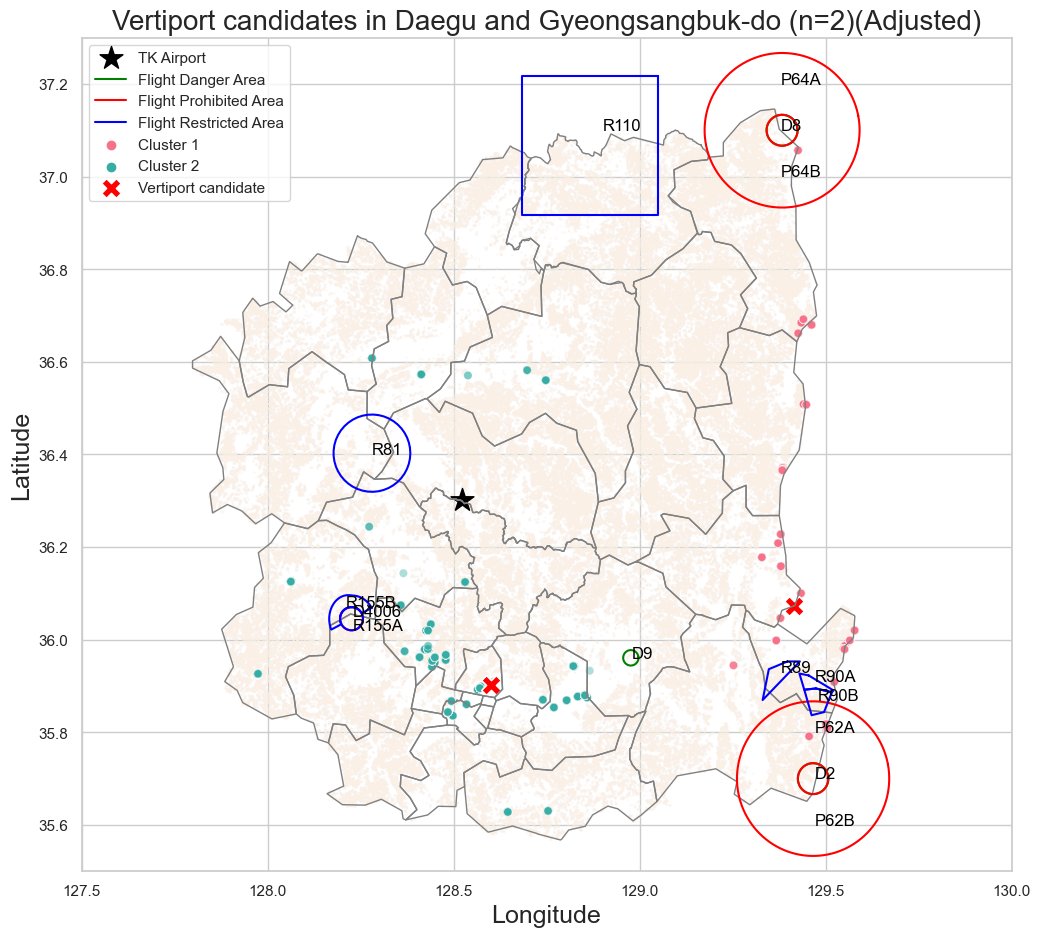
\includegraphics[width=\linewidth]{figure/K2.png}
      \end{minipage}%
      \begin{minipage}{0.5\textwidth}
        \centering
        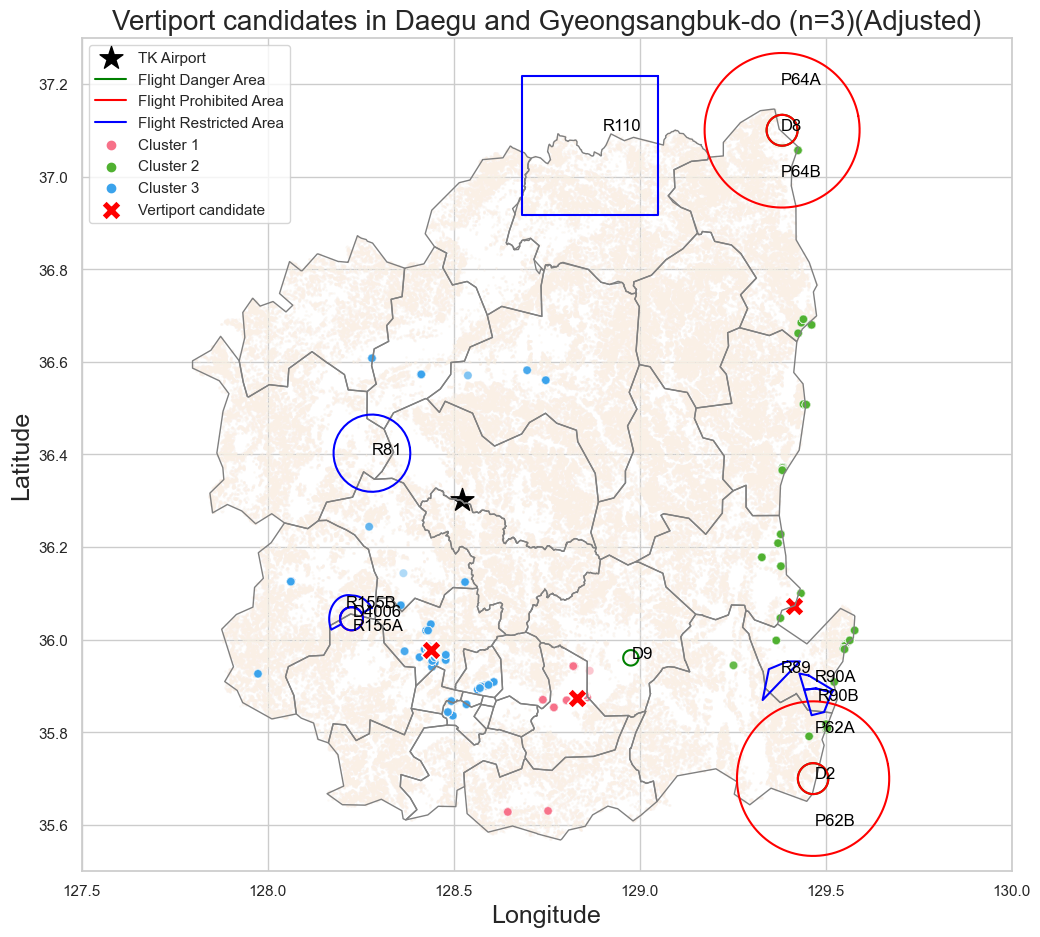
\includegraphics[width=\linewidth]{figure/K3.png}
      \end{minipage}%
      \caption{Vertiport candidates determined by K-means algorithm (K = 2 and K = 3)}
      \label{fig:overall}
    \end{figure}

    \begin{figure}[H]
      \centering
      \begin{minipage}{0.5\textwidth}
        \centering
        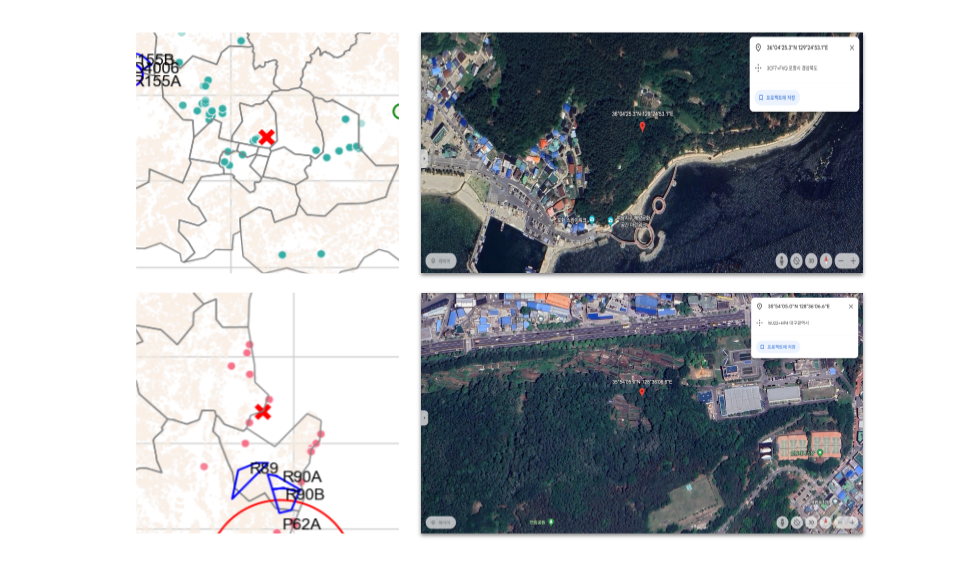
\includegraphics[width=\linewidth]{figure/K2_gm.png}
      \end{minipage}%
      \begin{minipage}{0.5\textwidth}
        \centering
        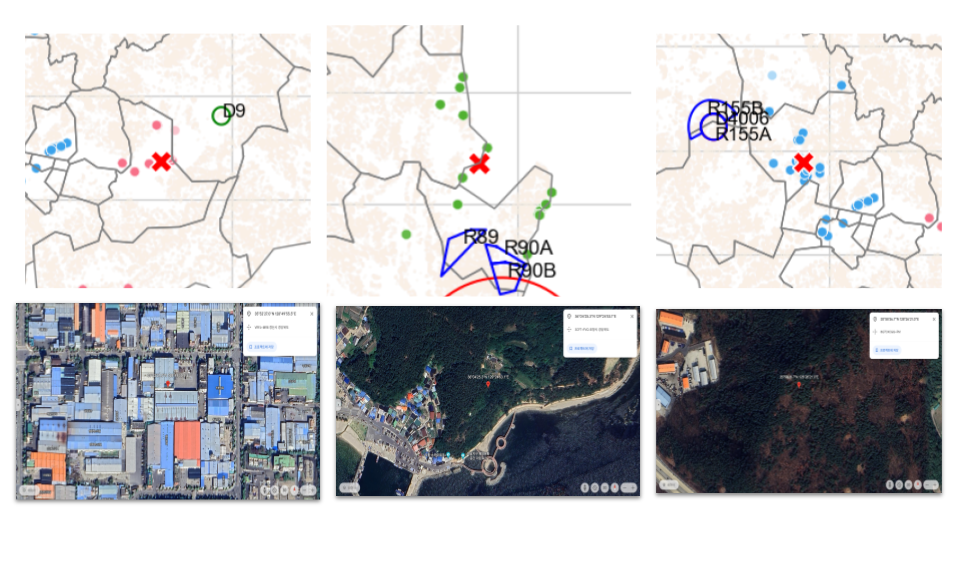
\includegraphics[width=\linewidth]{figure/K3_gm.png}
      \end{minipage}%
      \caption{Vertiport candidates determined by K-means algorithm (K = 2 and K = 3)}
      \label{fig:overall}
    \end{figure}

    
    \subsection{Validation strategy}
    There are two hypotheses set in our study: 1. There is a positive correlation between Logistic Demand and Logistic warehouse volume. 2. Vertiport placement candidates selected by the K-Means algorithm will reduce logistics delivery time. To validate the two hypotheses set by our team, we take the following steps. \

    For the first hypothesis - There is a positive correlation between logistic demand and logistic warehouse volume - we utilize the logistic demand and logistic warehouse volume datasets from Hwasung, provided CJ Logistics. Setting logistic demand as the dependent variable and warehouse volume as the independent variable we can derive a simple linear regression equation and derive a non-zero, positive-gradient logistic regression equation, which supports our hypothesis. Utilizing the regression equation, we can further infer the logistic demand dataset from other provinces/regions via warehouse volume. Visualization of hypothesis 1 validation is illustrated in Figure 6. \\

     \begin{figure}[H]
        \centering
        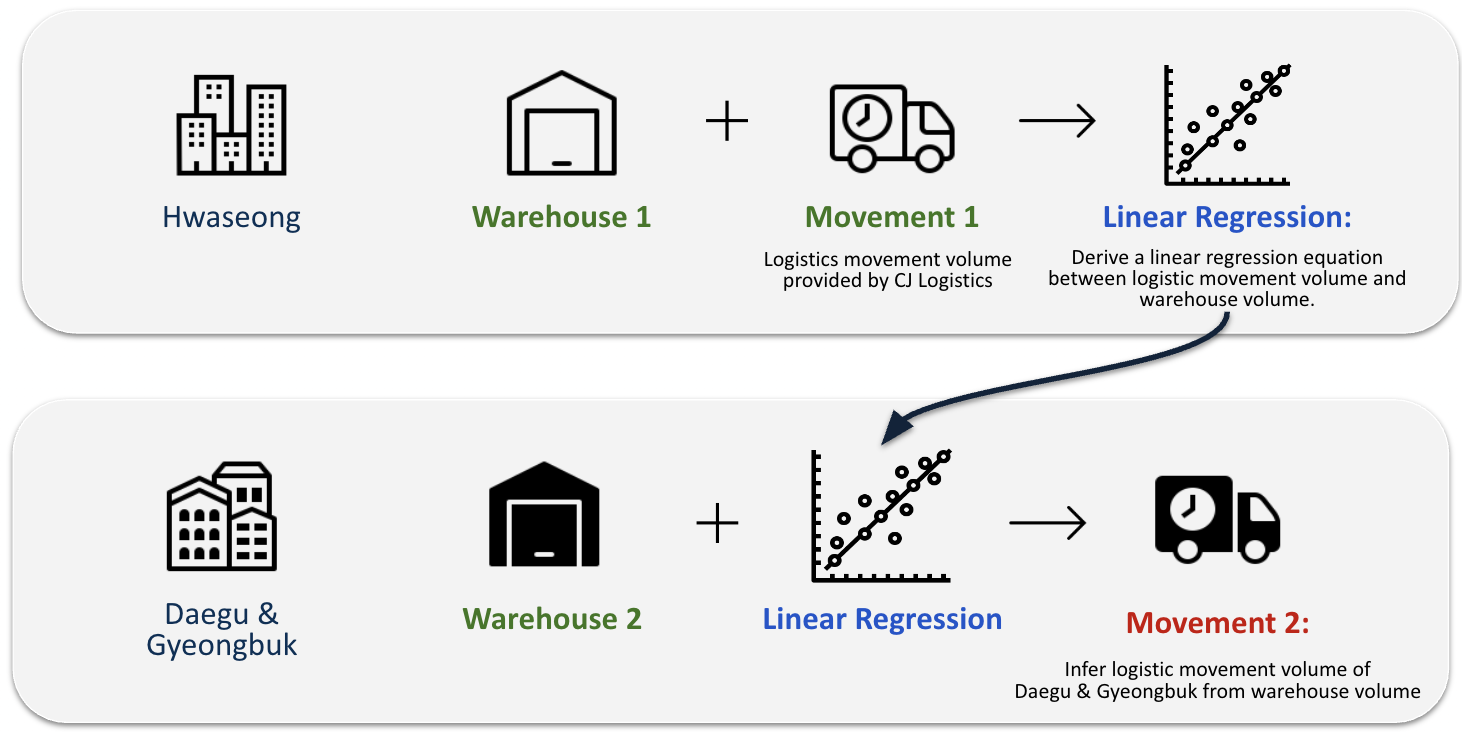
\includegraphics[width = 8cm]{./figure/hypothesis1.png}
        \caption{Hypothesis 1}
        \label{fig:enter-label}
    \end{figure}
    \\

    For the second hypothesis, we will calculate the time taken for two different approaches to transport from one location to another. The first approach is a simple, and direct travel from the Gunwi airport to Handong Global University via KIA's 'Bongo 3' vehicle. On the other hand, the second approach consists of traveling from the Gunwi airport to the vertiport station via the vehicle 'Alia250' and from the vertiport station to Handong Global University, via KIA's 'Bongo3' vehicle. The comparison of the two approaches is illustrated in Figure 7. We estimate the travel time of Bongo 3 by using a Kakao map's navigation system and as for Alia250, we assume that it travels linearly at the speed of 80\% of its maximum speed.\\
    
    \begin{figure}[H]
        \centering
        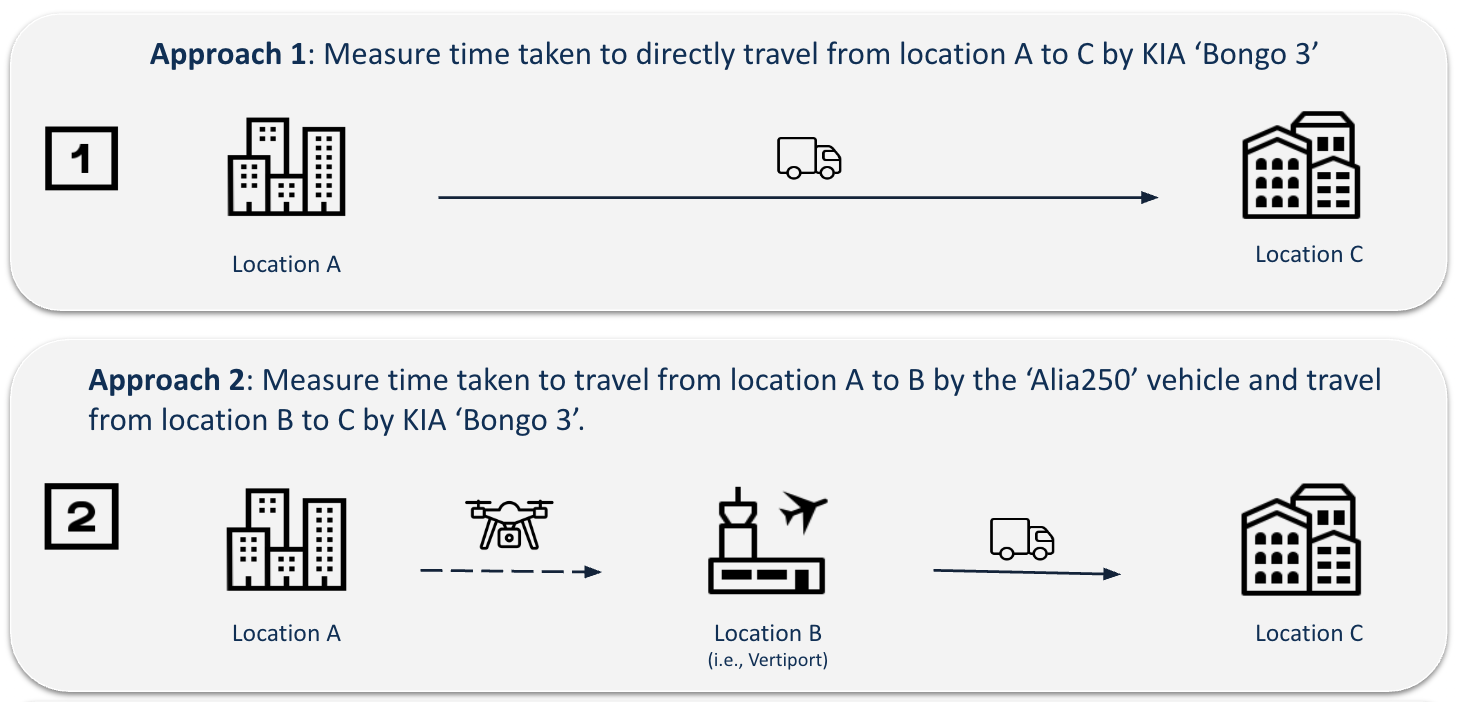
\includegraphics[width = 8cm]{./figure/hypothesis2.png}
        \caption[width = 10cm]{Hypothesis 2}
        \label{fig:enter-label}
    \end{figure}

    \section{Expected results}   

    In our research project, by using the K-means clustering algorithm, we aimed to determine the optimal vertiport locations in Gyeongsangbuk-do \& Daegu and achieved approximately 50\% reduction in delivery time.
    
    The result of this project can be used for Logistics companies aiming for efficient delivery by introducing UAM into their transportation system, to identify strategic locations of vertiports to enhance the efficiency of the middle-mile delivery system for fresh food.
    
    The outcomes of our project also can be used by city planners in Gyeongsangbuk-do and Daegu who want to optimize the middle-mile delivery system using UAM for the upcoming opening of the new TK airport distribution hub.

    Theoretically, the pipeline of our project can be expanded to other cold-chain products such as medicine by changing the data points of the warehouse into hospitals.\\   
    
    \bibliographystyle{apalike} % apalike 
    \bibliography{proposal_bib}

\end{document}
